\begin{custom-simple}[Problem 17]
\begin{center}
    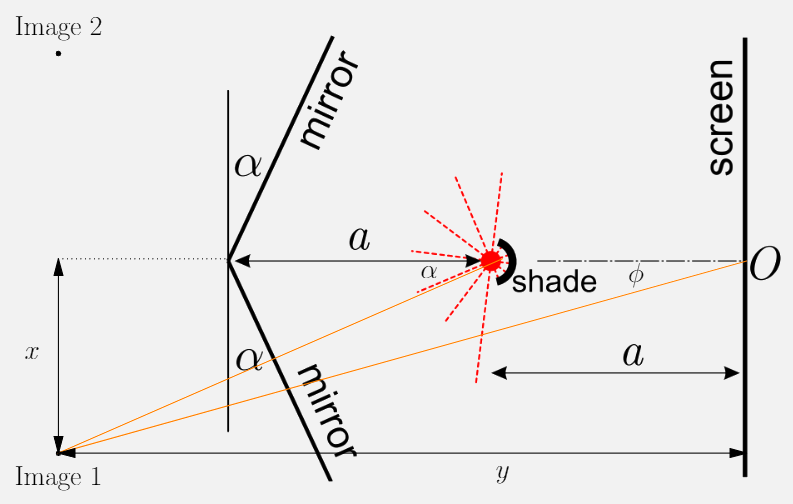
\includegraphics[width=12cm]{p17.png}
\end{center}
We find the images of light source in the mirrors. The light incident around $O$ can then be viewed as a superposition of the light emitted from the images. Let us take the line joining point $O$ and the point of intersection as x-axis and the line perpendicular to x-axis and passing through point $O$ as y-axis. Position of the image formed by the lower mirror is
$$y&=-2a\cos\alpha\sin\alpha, x=-2a\cos\alpha\cos\alpha + a$$
$$ \tan \phi &= \frac {y}{x} = \frac {2a\cos\alpha\cdot \sin\alpha}{2a\cos\alpha\cdot \cos\alpha + a}, \sin \phi = \frac {\tan \phi}{\sqrt {1 + (\tan \phi)^2}}$$
$$\sin \phi = \frac{\sin 2\alpha}{\sqrt {8\cos^2\alpha + 1}}$$
Let some point $M$ near point $O$ be the point of constructive interference. If we move up from this point by distance $d$, the path of light from the lower image would be increased by $d \sin\phi$ and the path of light from the upper image would be shortened by $d \sin\phi$. So we get a path difference $2d \sin\phi$ compared to $M$. This is again a point of constructive interference if $\lambda = 2d \sin\phi$. So we get the answer
$$\lambda = \frac{2d \sin 2\alpha}{\sqrt{8\cos^2\alpha + 1}}$$
\end{custom-simple}